\documentclass[10pt]{article}\usepackage[]{graphicx}\usepackage[]{color}
%% maxwidth is the original width if it is less than linewidth
%% otherwise use linewidth (to make sure the graphics do not exceed the margin)
\makeatletter
\def\maxwidth{ %
  \ifdim\Gin@nat@width>\linewidth
    \linewidth
  \else
    \Gin@nat@width
  \fi
}
\makeatother

\definecolor{fgcolor}{rgb}{0.345, 0.345, 0.345}
\newcommand{\hlnum}[1]{\textcolor[rgb]{0.686,0.059,0.569}{#1}}%
\newcommand{\hlstr}[1]{\textcolor[rgb]{0.192,0.494,0.8}{#1}}%
\newcommand{\hlcom}[1]{\textcolor[rgb]{0.678,0.584,0.686}{\textit{#1}}}%
\newcommand{\hlopt}[1]{\textcolor[rgb]{0,0,0}{#1}}%
\newcommand{\hlstd}[1]{\textcolor[rgb]{0.345,0.345,0.345}{#1}}%
\newcommand{\hlkwa}[1]{\textcolor[rgb]{0.161,0.373,0.58}{\textbf{#1}}}%
\newcommand{\hlkwb}[1]{\textcolor[rgb]{0.69,0.353,0.396}{#1}}%
\newcommand{\hlkwc}[1]{\textcolor[rgb]{0.333,0.667,0.333}{#1}}%
\newcommand{\hlkwd}[1]{\textcolor[rgb]{0.737,0.353,0.396}{\textbf{#1}}}%
\let\hlipl\hlkwb

\usepackage{framed}
\makeatletter
\newenvironment{kframe}{%
 \def\at@end@of@kframe{}%
 \ifinner\ifhmode%
  \def\at@end@of@kframe{\end{minipage}}%
  \begin{minipage}{\columnwidth}%
 \fi\fi%
 \def\FrameCommand##1{\hskip\@totalleftmargin \hskip-\fboxsep
 \colorbox{shadecolor}{##1}\hskip-\fboxsep
     % There is no \\@totalrightmargin, so:
     \hskip-\linewidth \hskip-\@totalleftmargin \hskip\columnwidth}%
 \MakeFramed {\advance\hsize-\width
   \@totalleftmargin\z@ \linewidth\hsize
   \@setminipage}}%
 {\par\unskip\endMakeFramed%
 \at@end@of@kframe}
\makeatother

\definecolor{shadecolor}{rgb}{.97, .97, .97}
\definecolor{messagecolor}{rgb}{0, 0, 0}
\definecolor{warningcolor}{rgb}{1, 0, 1}
\definecolor{errorcolor}{rgb}{1, 0, 0}
\newenvironment{knitrout}{}{} % an empty environment to be redefined in TeX

\usepackage{alltt}

\usepackage{amsmath,amssymb,amsthm}
\usepackage{fancyhdr,url,hyperref}
\usepackage{graphicx,xspace}
\usepackage{subfigure}
\usepackage{tikz}
\usetikzlibrary{arrows,decorations.pathmorphing,backgrounds,positioning,fit,through}

\oddsidemargin 0in  %0.5in
\topmargin     0in
\leftmargin    0in
\rightmargin   0in
\textheight    9in
\textwidth     6in %6in
%\headheight    0in
%\headsep       0in
%\footskip      0.5in

\newtheorem{thm}{Theorem}
\newtheorem{cor}[thm]{Corollary}
\newtheorem{obs}{Observation}
\newtheorem{lemma}{Lemma}
\newtheorem{claim}{Claim}
\newtheorem{definition}{Definition}
\newtheorem{question}{Question}
\newtheorem{answer}{Answer}
\newtheorem{problem}{Problem}
\newtheorem{solution}{Solution}
\newtheorem{conjecture}{Conjecture}

\pagestyle{fancy}

\lhead{\textsc{Prof. McNamara}}
\chead{\textsc{SDS/MTH 220: Lecture notes}}
\lfoot{}
\cfoot{}
%\cfoot{\thepage}
\rfoot{}
\renewcommand{\headrulewidth}{0.2pt}
\renewcommand{\footrulewidth}{0.0pt}

\newcommand{\ans}{\vspace{0.25in}}
\newcommand{\R}{{\sf R}\xspace}
\newcommand{\cmd}[1]{\texttt{#1}}

\rhead{\textsc{September 18, 2017}}
\IfFileExists{upquote.sty}{\usepackage{upquote}}{}
\begin{document}

\paragraph{Agenda}
\begin{enumerate}
  \itemsep0em
  \item Univariate Distribution
  \item Bivariate Relationships
  \item Correlation
\end{enumerate}

\paragraph{Univariate Distribution}

Let's review the graphics and statistics we could use to describe one variable.
\begin{itemize}
\itemsep5em
\item Quantitative variables
\item Categorical variables
\end{itemize}
\vspace{5em}

\paragraph{Bivariate Relationships}

\begin{itemize}
  \itemsep0em
  \item Response variable (aka dependent variable): the variable that you are trying to understand
  \item Explanatory variable (aka independent variable, aka predictor): the variable that you can measure that you think might be related to the response variable
  \item Graphics: Put response variable on $y$-axis and explanatory variable on $x$-axis
  \begin{itemize}
    \item Two quantitative variables: scatterplot [\cmd{qplot()} or \cmd{geom\_point()}]  
    \begin{itemize}
      \item Overall patterns and deviations from those patterns
      \item Form (e.g. linear, quadratic, etc.), direction (positive or negative), and strength (how much scatter?)
      \item Outliers
    \end{itemize}
    \item Quantitative response and a categorical explanatory variable:
    \begin{itemize}
      \item Side-by-side box plots [\cmd{geom\_boxplot()}]
      \item Multiple density plots [\cmd{geom\_density()} with \cmd{color} aesthetic or \emph{facets}]
    \end{itemize}
    \item Two categorical variables: mosaic plot [\cmd{mosaicplot()}]: 
    \item If a third categorical variable exists, use the \cmd{color} option or facets
  \end{itemize}
  \item Correlation: numerical measure of direction and strength of a \emph{linear} relationship!
\end{itemize}

\begin{knitrout}
\definecolor{shadecolor}{rgb}{0.969, 0.969, 0.969}\color{fgcolor}\begin{kframe}
\begin{alltt}
\hlkwd{require}\hlstd{(mosaic)}
\hlkwd{qplot}\hlstd{(}\hlkwc{data} \hlstd{= KidsFeet,} \hlkwc{y} \hlstd{= length,} \hlkwc{x} \hlstd{= width)}
\hlkwd{qplot}\hlstd{(}\hlkwc{data} \hlstd{= KidsFeet,} \hlkwc{y} \hlstd{= length,} \hlkwc{x} \hlstd{= sex,} \hlkwc{geom} \hlstd{=} \hlstr{"boxplot"}\hlstd{)}
\hlkwd{qplot}\hlstd{(}\hlkwc{data} \hlstd{= KidsFeet,} \hlkwc{x} \hlstd{= length,} \hlkwc{color} \hlstd{= sex,} \hlkwc{geom} \hlstd{=} \hlstr{"density"}\hlstd{)}
\hlkwd{qplot}\hlstd{(}\hlkwc{data} \hlstd{= KidsFeet,} \hlkwc{x} \hlstd{= length,} \hlkwc{facets} \hlstd{=} \hlopt{~}\hlstd{sex,} \hlkwc{geom} \hlstd{=} \hlstr{"density"}\hlstd{)}
\hlkwd{mosaicplot}\hlstd{(domhand} \hlopt{~} \hlstd{sex,} \hlkwc{data} \hlstd{= KidsFeet)}
\end{alltt}
\end{kframe}
\end{knitrout}

\newpage

\paragraph{Correlation}

The (Pearson Product-Moment) correlation coefficient [\cmd{cor()}] is a measure of the strength and direction of the \emph{linear} relationship between two numerical variables. It is usually denoted $r$ and is measured on the scale of $[-1, 1]$. 

\begin{knitrout}
\definecolor{shadecolor}{rgb}{0.969, 0.969, 0.969}\color{fgcolor}\begin{kframe}
\begin{verbatim}
## # A tibble: 4 x 5
##     set     N `mean(x)` `mean(y)` `cor(x, y)`
##   <chr> <int>     <dbl>     <dbl>       <dbl>
## 1     1    11         9  7.500909   0.8164205
## 2     2    11         9  7.500909   0.8162365
## 3     3    11         9  7.500000   0.8162867
## 4     4    11         9  7.500909   0.8165214
\end{verbatim}
\end{kframe}
\end{knitrout}

\begin{knitrout}
\definecolor{shadecolor}{rgb}{0.969, 0.969, 0.969}\color{fgcolor}\begin{kframe}
\begin{alltt}
\hlkwd{qplot}\hlstd{(}\hlkwc{data} \hlstd{= ds,} \hlkwc{x} \hlstd{= x,} \hlkwc{y} \hlstd{= y)} \hlopt{+}
  \hlkwd{geom_smooth}\hlstd{(}\hlkwc{method} \hlstd{=} \hlstr{"lm"}\hlstd{,} \hlkwc{se} \hlstd{=} \hlnum{0}\hlstd{)} \hlopt{+}
  \hlkwd{facet_wrap}\hlstd{(}\hlopt{~}\hlstd{set)}
\end{alltt}
\end{kframe}
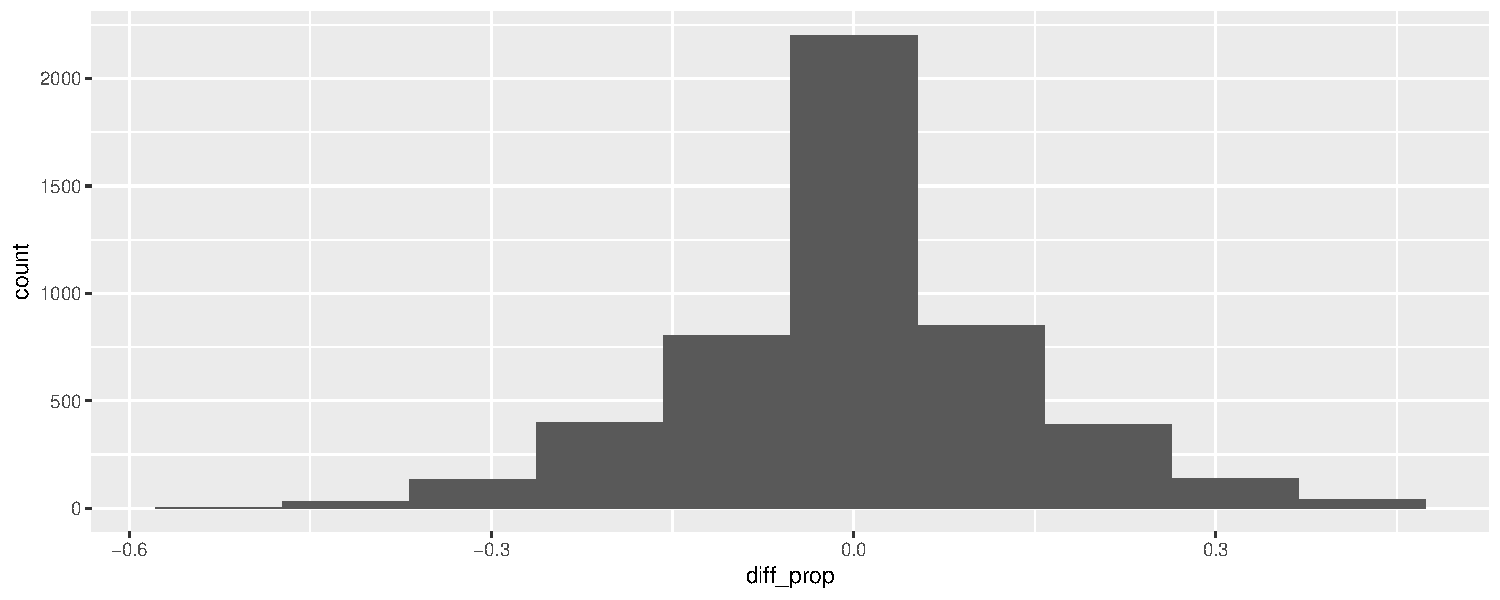
\includegraphics[width=\maxwidth]{figure/unnamed-chunk-3-1} 

\end{knitrout}





Note that correlation only measures the strength of a \emph{linear} relationship. In each of the four very different (\href{http://en.wikipedia.org/wiki/Anscombe%27s_quartet}{Anscombe}) data sets shown above, the correlation coefficient is the same (up to three digits)!

\paragraph{Examples}

Get a feel for the value of the correlation coefficient in \href{http://upload.wikimedia.org/wikipedia/commons/thumb/d/d4/Correlation_examples2.svg/1000px-Correlation_examples2.svg.png}{different scatterplots}.

\begin{enumerate}
  \item Do a \href{https://www.google.com/search?q=scatterplot&tbm=isch}{Google Image search for ``scatterplot"} and describe the form, direction, and strength of three different-looking patterns. Sketch each plot.
  \begin{enumerate}
    \itemsep1in
    \item :
    \item :
    \item :
    \vspace{0.5in}
  \end{enumerate}
\end{enumerate}


\end{document}
